\documentclass[parskip,
			twoside,
			longdoc,
			10pt,
			noheadingspace,
			accentcolor=tud0a,
			bigchapter,
			%draft,
			colorback]{tudreport}

%% Spracheinstellungen
\usepackage[english]{babel}
\usepackage[utf8]{inputenc}
\usepackage[T1]{fontenc} 
\usepackage{microtype} % optischer Randausgleich bei pdflatex mit Zeichendehnung
\DisableLigatures[-]{family=tt*}

%% Grafikeinstellungen
\usepackage{float} % u.a. genaue Plazierung von Gleitobjekten mit H
\usepackage{wrapfig}
%\setlength{\intextsep}{0pt}
%\addto\captionsngerman{%
%  \renewcommand{\figurename}{Abb.}%
%}
\usepackage{pgfplots}
\pgfplotsset{compat=1.3}
\usepackage{caption}

%% Tabelleneinstellungen
\usepackage{booktabs}
\usepackage{multirow}
\usepackage{longtable}
\usepackage{tabularx}

%% Mathematik
\usepackage{amsmath}
\usepackage{nicefrac}
\usepackage{icomma}

%% Code
%\usepackage{listings}
%\lstset{breaklines=true} 
%\usepackage{listings} 
	%\lstset{numbers=left, numberstyle=\tiny}  %, numbersep=2pt
	%\lstset{language=Perl}

%\usepackage{calc}
%\usepackage{etoolbox}
%\makeatletter
%\preto{\@verbatim}{\topsep=0pt \partopsep=0pt }
%\makeatother


%% sonstige Einstellungen
\usepackage{paralist}% erweiterte Listenumgebung (z.B. compactitem)
\usepackage{textcomp} % verschiedene Symbole
\usepackage{hyperref}
%\renewcommand\plparsep{1ex}

% Don't stretch spaces
\raggedbottom

\usepackage{enumerate}
\usepackage[acronym,toc]{glossaries}
%\renewcommand{\glsnamefont}[1]{\textbf{#1}}
\renewcommand{\glossaryname}{Acronyms}

\usepackage{makeidx}
\makeindex

\usepackage[fixlanguage]{babelbib}
\selectbiblanguage{english}


\title{Design of an Accelerated Event-based Server}
\subtitle{Bachelor Thesis by Peter Schuster}
\subsubtitle{January 2013}
%\setinstitutionlogo{ies-logo.pdf}
\institution{\textbf{Department of Electrical Engineering and Information Technology (ETiT)}\vspace{1mm}\\Institute of Computer Engineering\\Integrated Electronic Systems Lab\\Prof. Dr.-Ing. Klaus Hofmann}
%\settitlepicture{images/spartan}

\setcounter{tocdepth}{1}

\lowertitleback{
\begin{addmargin}[.5in]{0cm}
Bachelor Thesis\\
\\
\begin{large}
\textbf{Design of an Accelerated Event-based Server}
\end{large}
\\
\\
submitted in partial fulfillment of the requirements \\
for the Degree of \textit{Bachelor of Science} \\
in \textit{Electrical Engineering and Information Technology}.
\\
\\
\\
Peter Schuster\\Darmstadt
\\
\\
\\
\begin{tabbing}
  \hspace{2.5cm} \= \kill
  Advisor: \> Dipl.-Ing. Boris Traskov \\
  Examiner: \> Prof. Dr.-Ing. Klaus Hofmann\\
\end{tabbing}
\vspace*{3mm}
\begin{tabbing}
  \hspace{4cm} \= \kill
  Start: \> 01/10/2012 \\
  \\
  Date of Submission: \> 02/01/2013 \\
  Date of Exam: \> 10/01/2013 \\
\end{tabbing}
\vspace*{5cm}
\end{addmargin}
}

\begin{document}

%% Titel %%%%%%%%%%%%%%%%%%%%%%%%%%%%%%%%%%%%%%%%%%%%%%%%%%%%%%%%%%%%%%%%%%
\maketitle
\cleardoublepage

%% Vorgeplnkel %%%%%%%%%%%%%%%%%%%%%%%%%%%%%%%%%%%%%%%%%%%%%%%%%%%%%%%%%%%%%%
\pagestyle{empty}
\pagenumbering{none}

\cleardoublepage
\newpage

\thispagestyle{empty}
\markright{Declaration}
\cleardoublepage
\vspace*{9cm}

Herewith I declare, that I have made the presented paper myself and solely with the aid of the means permitted by the examination regulations of the Darmstadt University of Technology.
The literature used is indicated in the bibliography.
I have indicated literally or correspondingly assumed contents as such.

\vspace*{3cm}

Darmstadt, September 2012\\

\vspace*{5mm}


\parbox{7cm}{\hrulefill}\\
\hspace*{0,3cm} Peter Schuster

\cleardoublepage
\endinput



% include glossary

%
% Glossary
%

%\newglossaryentry{FPGA}{Field Programmable Gate Array}
\newacronym{fpga}{FPGA}{Field Programmable Gate Array}

\cleardoublepage
\tableofcontents

%\newpage
%\phantomsection %notwendig, damit Link nicht unterhalb der Überschrift zeigt
%\addcontentsline{toc}{chapter}{List of figures}
%\listoffigures

\pagenumbering{arabic}

%% Hauptteil %%%%%%%%%%%%%%%%%%%%%%%%%%%%%%%%%%%%%%%%%%%%%%%%%%%%%%%%%%%%%%%
\pagestyle{headings}

\cleardoublepage
\chapter{Einleitung}

Das Projektseminar steht im Kontext der Forschung an High-Performance Netzwerkkarten zur Übertragung von Daten mit bis zu 40 GB/s. TCP Offload Engine

\section{Ziel}

Ziel des Projektseminars ist es einen \ac{FPGA} zu programmieren um über eine Ethernet-Schnittstelle Daten zwischen dem Evaluationsboard und einem weiteren Gerät auszutauschen und Lasttests durchzuführen.

\section{Testumgebung}

Für die Versuche, Messungen und Tests wird das Evaluationsboard ML505 von XILINX verwendet. Die Programmierung des \ac{FPGA} erfolgt über das \textit{Xilinx ISE Studio}, bzw. \textit{Xilinx SDK}.



\chapter{Implementierung}

\chapter{Evaluation}

\chapter{Ausblick}
\chapter{System Requirements}

Requirements for the designed system must be collected with two key points in mind: the desired outcome of the project and the chosen/available hardware system and tool set.

Objective of the project is to run \textit{nginx}, an event-based web server. \textit{nginx} can not be executed directly on the processor, because it requires the presence of an an \gls{os} providing a file system and taking responsibility of process and thread management. 

\textit{nginx} supports a number of free (FreeBSD, Solaris, Linux) and proprietary (AIX, HP-UX) unix-based operating systems, as well as \textit{Microsoft Windows}.\footnote{see \url{http://nginx.org/en/\#tested_os_and_platforms}}

\textit{Microsoft Windows} is currently only available for Intel's \textit{x86} and AMD's \textit{AMD64} (also known as \textit{x86-64}) architectures. The constraint on the available \textit{Xilinx XC5VLX110T} \gls{fpga} demands an easy-to-implement, low cost microprocessor system. But the mentioned processor architectures do not count towards these categories. Therefore the choices are limited to free unix-based operating systems.

Due to the by far largest number of supported processor architectures and wide distribution, the choice was made to go with Linux as operating system for the project.

Linux demands a \gls{mmu} in virtual mode and two memory protection zones.\footnote{Linux kernel can be configured for processors without \gls{mmu}, but this is not recommended.} \gls{mmu}s enable an \gls{os} "to exercise a high degree of
management and control over its address space and the address space it allocates to processes" \cite{linuxPrimer}[sec. 2.3.5]. Linux kernel furthermore requires the presence of two timers and an interrupt controller.\footnote{see \url{http://wiki.xilinx.com/microblaze-linux\#toc4}, as of 09/07/2012}

The used web server software (\textit{nginx}) requires the availability of an event module in the \gls{os}. Linux kernel contains a number of event modules, all being supported by \textit{nginx}. The preferred and most effective one is \textit{epoll}.\footnote{\url{http://wiki.nginx.org/NginxOptimizations} (as of 12/2012)}
\chapter{Preceding Work}

Preceding to this bachelor thesis, a project seminar with the same title was taken. During this project seminar the first part of the project was implemented. The outcome of this project seminar is described in the following chapter. A detailed description on how this was accomplished can be found in the respecting project report \cite{projectseminar}.

\section{The Hardware System}

\subsection{Architecture}

In this project a \gls{soc} was build on top of a \gls{fpga} using predefined \gls{ip} cores for the processor and additional system components.

An overview of the complete hardware architecture of the system described in the next sections is included in the appendix of this report (\ref{sec:hw_arch}).

\subsubsection{Processor}
\label{subsubsec:microblaze}

The used \textit{XC5VLX110T} \gls{fpga} does not have a build-in hard core processor, therefore a single core \textit{MicroBlaze} soft core processor was chosen. The \textit{MicroBlaze} processor is a proprietary processor, developed by \textit{Xilinx} for their \gls{fpga} families and supported by the Xilinx hard- and software development kits. Its design follows the Harvard architecture with separate data and instruction memory.

Running Linux kernel requires the presence of a \gls{mmu}. To improve the system performance instruction and data caches (16 KB), barrel shifter, multiplier (64 bit) and the hardware division modules were enabled.

\subsubsection{Bus System}

For connecting the \textit{MicroBlaze} processor to other peripherals on the chip the \gls{plb}, invented by \textit{IBM} as part of the \textit{CoreConnect} bus system, was selected.

Prior to the \textit{Virtex-6} \gls{fpga} family, only this bus system was available. \textit{Virtex-6} \gls{fpga}s support also the \gls{axi} system, which is part of the \gls{amba}, designed by \textit{ARM}, but the used \textit{Xilinx XC5VLX110T} \gls{fpga} is part of the \textit{Virtex-5} family, therefore \gls{plb} needed to be selected as interconnect type. \cite{axi_interconnect}[p. 1, facts table]

\subsubsection{Memory}

\textit{XUPV5-LX110T} boards contain a single-rank unregistered 256 MB DDR2 SODIMM, which is connected to the processor via a memory controller. This memory controller is implemented in the \textit{Multi-Port Memory Controller} (MPMC) \gls{ip} core. The memory base address was set to \texttt{0x50000000}.

\subsubsection{Network Interface}

The \textit{Xilinx XC5VLX110T} \gls{fpga} has four \textit{Tri-Mode Ethernet Media Access Controllers}, designed to the IEEE 802.3-2002 specification, operating at 10, 100, and 1,000 Mb/s. \cite{virtex5}[p. 4, table 1] To use these hard core controllers an \texttt{xps\_ll\_temac} soft IP core was added to the \gls{soc}, acting as a wrapper for the hard core to integrate it into the system.


\gls{gmii} as a backwards compatible extension to \gls{mii} supporting data rates of up to 1,000 Mb/s was selected as physical interface type, because support for Gigabit Ethernet was desired, but there was no need for a reduced data path width. Therefore the jumpers \texttt{J22} and \texttt{J23} on the \textit{Xilinx XUPV5} board need to be set to positions \texttt{1-2} to enable \gls{gmii} as physical interface type.

Usage of an integrated checksum calculation circuit is enabled on the system, using the parameters \texttt{C\_TEMAC0\_TXCSUM} and \texttt{C\_TEMAC0\_RXCSUM}.

\subsection{Clocks}
\label{sec:clocks}

Clocks for the system are generated using a \textit{clock\_generator} \gls{ip} core, with an external oscillator providing a 100 MHz clock. \cite{ug347}[p. 20]

Due to high delays on data paths in the decode pipeline stage, a clock period of at least \textit{9.12 ns} is required, resulting in a system clock frequency for the processor and local bus of 100 MHz.

The memory controller (MPMC) is driven by base clock of 200 MHz, a clock with half the frequency of the base clock (100 MHs) and a 200 MHz clock signal, shifted by 90°. All these clock signals are controlled by the same \gls{pll} used by the system clock signal.

The \texttt{GTX\_CLK} port of the Ethernet \gls{mac} \gls{ip} core is driven by a clock signal with exactly 125 MHz for operating \textit{GMII} (defined by the specifications of GMII \cite{ieee802_3}[sec. 35.2.2.1]). For \gls{dma} a clock signal with a frequency identical to the local bus clock is required. The \texttt{REFCLK} was connected to a 200 MHz clock, according to the respective manual of the \gls{ip} core \cite{xps_ll_temac}[p. 11, table 3].

\subsection{Endianness}

\begin{quote}
 "Endianness describes how multi-byte data is represented by a computer system and is dictated by the CPU architecture of the system." \cite{intel_endiannness}[p. 5]
\end{quote}

Architectures utilizing the little endian concept store the least significant byte (LSB) at the lowest address, in big endian architectures the most significant byte (MSB) is stored at the highest address. \cite{intel_endiannness}[p. 6]

Linux can be build for little, as well as for big endian systems. Only confinement is that the used toolchain (compiler, etc. - see \ref{subsec:sdk}) needs to support the endianness of the architecture.

The \textit{MicroBlaze} processor has the parameter \texttt{C\_ENDIANNESS} to specify the endianness of the processor. But although the \textit{MicroBlaze Processor Reference Guide} states that "the \texttt{C\_ENDIANNESS} parameter is automatically set to little endian when using AXI4, and to big endian when using PLB, but can be overridden by the user" \cite{mb_ref}[p. 52], this parameter must not be changed for \textit{Virtex-5} \gls{fpga}s. This is reasoned in the disability of the peripheral cores connected via \gls{plb}, to handle data other than in big endian byte order. The \gls{axi} bus circumvents this problem by swapping bytes.\footnote{\url{http://forums.xilinx.com/t5/EDK-and-Platform-Studio/Memory-Test-fails-for-8-and-16-bit/m-p/253922/highlight/true\#M23973} (in-official statement by a Xilinx employee)}

Therefore big endian was selected for the system architecture of this project.

\section{The Software}

\subsection{Linux Kernel}

Running Linux on a \textit{MicroBlaze} processor is unfortunately rarely documented and not wide spread. Mainly two projects exist on this topic: \textit{PetaLinux} and \textit{BlueCat Linux}. Unfortunately both were turned into commercial solutions and although the patched Linux source code is publicly available, it is hardly usable without the proprietary toolkit, documentation and support, sold by the companies driving these projects.

When talking about Linux, it needs to be distinguished between the Linux kernel as the actual \gls{os} and Linux distributions (like \textit{Ubuntu}, \textit{Debian}, \textit{openSUSE}, \textit{Fedora} and many more), containing additional libraries, applications and configuration. The Linux kernel in itself is the heart of a Linux installation. There exists one major development line (called "mainline"), being maintained by a group around the founder of Linux, Linus Torvalds. But there exist also also copies of the source code (called "fork") with incorporated custom changes.

Originally support for \textit{MicroBlaze} soft-core processors in the Linux kernel was developed by \textit{Xilinx} and \textit{PetaLogix} in an own fork of Linux kernel, but with version 2.6.30, released on the 9th of June 2009, their additions were merged into the mainline Linux kernel and the \textit{MicroBlaze} architecture is officially supported by Linux since this date.\footnote{\url{http://www.petalogix.com/news/microblaze-architecture-merged-into-kernel.org}} The still maintained and actively used source code repositories of \textit{Xilinx}\footnote{\url{http://git.xilinx.com/?p=linux-xlnx.git}} and \textit{PetaLogix}\footnote{\url{http://developer.petalogix.com/git/gitweb.cgi?p=linux-2.6-microblaze.git}} contain some further additions to device drivers and unreleased changes.

For this project the Linux kernel source code from the \textit{Xilinx} repository was taken. All development, additions and evaluation was done on top of commit \texttt{ed63a4d76efadcb68f5776e4244766ffea226cc4} (June, 18th 2012)\footnote{\url{http://git.xilinx.com/?p=linux-2.6-xlnx.git;a=commit;h=ed63a4d76efadcb68f5776e4244766ffea226cc4}} as part of version \texttt{3.3.0-14.2-build1}.

To enable correct recognition of the latest \textit{MicroBlaze} processor versions with enabled \gls{pvr} a patch included in the appendix of this report (\ref{subsec:pvr_patch}) needs to be applied to the Linux kernel sources. The patch was extracted from the \textit{PetaLogix} Linux kernel fork.

\subsection{Development Environment and Cross Compilation}
\label{subsec:sdk}

To build the Linux kernel a set of tools (called toolchain) compiling source code files and linking binary output in an executable file is required. This toolchain needs to meet two criteria: the architecture/\gls{os} it was build to run on top and the target architecture for which images are compiled and linked. Building an image with a different target architecture, than the architecture of the executing system, is called \textit{cross compilation}. Because it is not practically possible to build the Linux kernel on a \textit{MicroBlaze} processor, without an existing and running \gls{os} on the \textit{MicroBlaze} system, a toolchain for cross compiling Linux kernel source from an existing, easily-usable system for a \textit{MicroBlaze} system, is needed. \textit{Xilinx} provides toolchains, based on the widely used \gls{gcc} and \textit{binutils}, for cross compiling from Linux x86 and x86-64 architectures to \textit{MicrobBlaze} systems as target architecture. For compiling the latest Linux kernel sources, version two of the toolchain containing \gls{gcc} in version 4.1.2 is required. This version of the toolchain itself requires a 64-bit Linux \gls{os} and can be downloaded from the \textit{Xilinx} source code repositories.\footnote{\url{http://git.xilinx.com/?p=xldk/microblaze_v2.0.git}}

During this project a virtual Linux machine with \textit{Ubuntu 12.04 64-bit} was used for all software development.

To enable cross compilation of the Linux kernel, two environment variables need to be set. The \texttt{CROSS\_COMPILE} variable specifies a prefix for all build tools. This is required, because on cross compilation there is usually more than one compiler available on the executing system. Furthermore the path to the utilized build tools needs to be added to the \texttt{PATH} variable.

The \texttt{ARCH} variable enables the inclusion of code specific to the target architecture. This code files reside in \texttt{/arch/<ARCH>/} inside the Linux kernel source folder. 

A build process is triggered by calling the \texttt{make} executable inside of the Linux kernel source folder.

\subsubsection{The Linux Configuration System}

Linux kernel consists of many optional sub-parts for target architectures, device drivers, special features, etc. Which of these parts are compiled and linked into the Linux kernel binary image needs to be configured in the \texttt{.config} file in the Linux kernel root directory. This file is "the configuration blueprint for building a Linux kernel image" \cite{linuxPrimer}[sec. 4.3.1] containing all (required) settings.

Although possible, it is not recommended to edit the \texttt{.config} file manually, because of many non-trivial dependencies among different configuration settings. Instead one of the available editors (\textit{menuconfig}, \textit{xconfig} and \textit{gconfig}) should be used. Because of its search capabilities inside the configuration settings, \textit{xconfig} was used as configuration editor during this project.\footnote{\textit{xconfig} requires the \textit{QT} library which can be installed through the package \texttt{qt4-dev-tools} on Debian and Ubuntu distributions.}

In the Linux kernel fork maintained by \textit{Xilinx} a base configuration for the \textit{ML507} board is included. It is recommended to use this configuration as base line instead of starting from scratch.

\subsubsection{Required Configuration Settings}
\label{subsubsec:req_config}

As discussed in \ref{subsubsec:microblaze}, the \textit{MicroBlaze} processor can be configured with different feature sets (multiplier, barrel shifter, etc.). Therefore the \gls{gcc} compiler needs to be parameterized for matching the provided features of the target system \cite{mb_linux}[sec. "Kernel Configuration Details"]. These need to be set in the \texttt{XILINX\_MICROBLAZE0\_*} settings inside of the \texttt{.config} file.

It is important to check that the \texttt{KERNEL\_BASE\_ADDR} setting is in line with the configured base address of the main memory (\texttt{C\_MPMC\_BASEADDR}) in the \textit{\gls{mhs}} file.

For inclusion of the driver for the \texttt{xps\_ll\_temac} \textit{\gls{ip} core}, the configuration option \texttt{XILINX\_LL\_TEMAC} needs to be enabled. Support for \textit{UART} device drivers can be enabled by the settings \texttt{SERIAL\_UARTLITE}, \texttt{SERIAL\_UARTLITE\_CONSOLE}, \texttt{SERIAL\_CORE} and \texttt{SERIAL\_CORE\_CONSOLE}, but this is already included in the default \textit{ML507} configuration settings provided by \textit{Xilinx}.

When there is no \textit{boot loader} triggering Linux kernel start, command-line options for the boot process need to be compiled into the Linux kernel image. Therefore the configuration setting \texttt{CMDLINE} exists.

Additionally some features like \textit{IPv6} support and various security algorithms were enabled in the Linux kernel configuration. The complete \texttt{.config} file with all settings is referenced in the report appendix.

\subsubsection{Device Tree}
\label{subsubsec:device_tree}

To avoid compiling all information about the target hardware system into assembler code, an abstraction called \textit{Device Tree} was invented. \textit{Device Tree} is the successor of \textit{IBM's} \textit{Open Firmware (OF)} and the flattened device tree, containing information about the hardware system like available feature sets and bus addresses. \cite{device_tree} It is accessed by the Linux kernel during the boot process for configuring itself and on lookup of hardware information. The \textit{Device Tree Source (dts)} file is compiled by the \textit{Device Tree Compiler (dtc)} during the Linux kernel build process to an \textit{Device Tree Blob (dtb)} and linked into the final Linux kernel image.

The \textit{dts} file must reside inside of the \texttt{arch/microblaze/boot/dts} directory (e.g. "\texttt{arch/microblaze/boot/dts/xupv.dts}") and can be specified on starting the Linux kernel build process (e.g. "\texttt{make ARCH=microblaze simpleImage.xupv5}").

A \textit{dts} file can be generated using the \textit{Device Tree Generator}, a \gls{tcl} script reading a system specification generated by \gls{xps} (see "SDK Export"). The latest version (1.3) of the \textit{Device Tree Generator}, maintained by Michal Simek, is referenced in the appendix of this report (\ref{subsec:dts-generator}).

Apart from the generated device information, the \textit{dts} file also contains options which must be set manually. These include an \texttt{aliases} node for mapping device instances to standardized interface names (\texttt{ethernet0} and \texttt{serial0}) and command-line options, overriding\footnote{By setting the kernel configuration option \texttt{CMDLINE\_FORCE} to "\texttt{y}", the command-line options specified in the \texttt{.config} file take precedence.} the ones specified in the Linux kernel configuration file.

Besides the options already explained in the "\textit{Required Configuration Settings}" section (\ref{subsubsec:req_config}), this configuration assigns the logical IPv4 address \texttt{192.168.3.10} to the network interface of the board.

The \textit{Device Tree Generator} can be setup as own \gls{bsp} inside of the \textit{Xilinx SDK}. A documentation with all required steps for setting it up can be found on the respective site hosted by \textit{Xilinx}.\footnote{\url{http://wiki.xilinx.com/device-tree-generator}}


\subsection{The File System}
\label{subsec:fs}

Although possible, it makes little sense to use the Linux kernel without a file system. Therefore one of the last steps in the boot process is the initialization of a \textit{root file system (rootfs)}. \cite{linuxPrimer}[sec. 6.1] On modern desktop and server systems this \textit{rootfs} is usually just a bare minimum file system, containing all necessary files to boot the Linux kernel, mounting a file system located on a hard drive or flash memory right after booting up. But the used system in this project has no hard drive attached, neither is one required for the purpose of the project, at the moment. Therefore we will stick with the initial \textit{rootfs} as the main file system.

A simple way to provide an initial \textit{rootfs} is the \textit{Initial RAM Disk (initrd)}. This is a file system packed in a \textit{cpio} archive and linked into the Linux kernel image. It is unpacked completely into the main memory during kernel boot process. \textit{Xilinx} provides two packed file system archives for a \textit{MicroBlaze} system within their Linux kernel repository: \texttt{initramfs\_minimal.cpio.gz} and \texttt{initramfs\_complete.cpio.gz}. Both contain all files and structures sufficient for this project. The archives can be linked into the Linux kernel image by setting the configuration option \texttt{INITRAMFS\_SOURCE} to one of the file names, respectively.

\textit{cpio} archives can be unpacked using the following command. This command should be executed as privileged root user to allow the creation of node points, used in the file system.

After all changes were made to the files representing the file system, it can be packed into a \textit{cpio} archive using the bash script supplied in the appendix of this report ("\texttt{pack-fs.sh}", \ref{subsec:pack-fs}). The paths to the Linux kernel sources and file system root need to be adjusted to meet the current environment.

\subsection{Deployment and Debugging}

The generated \textit{bitstream} of the hardware system representing the \gls{soc}, needs to be programmed into the \gls{fpga} on every power-on. This is required, because the configuration of the \gls{fpga} being set by the \textit{bitstream} is volatile. Programming the \textit{bitstream} is straight forward and can be accomplished using the \textit{Xilinx iMPACT} tool, which is part of the \textit{Xilinx ISE Design Suite}.

When the Linux kernel build is finished, the resulting \textit{\gls{elf}} file can be found at \texttt{arch/microblaze/boot/simpleImage.<dts-name>}. This file can be loaded into the \gls{fpga} using \textit{\gls{xmd}}, which is also part of the \textit{Xilinx ISE Design Suite}. The steps for loading an \gls{elf} file onto a \gls{fpga} with \textit{MicroBlaze} processor using \gls{xmd} are as follows:

\begin{enumerate}
  \setlength{\itemsep}{1pt}
  \setlength{\parskip}{2pt}
  \setlength{\parsep}{0pt}
\item Connecting to the \textit{MicroBlaze} processor:\\ \texttt{xmd> connect mb mdm}
\item Stopping the \textit{MicroBlaze} processor:\\ \texttt{xmd> stop}
\item Downloading the \gls{elf} file:\\ \texttt{xmd> dow simpleImage.<dts-name>}
\item Starting the \textit{MicroBlaze} processor:\\ \texttt{xmd> con}
\end{enumerate}

After committing these steps the Linux kernel boot log should be written to the connected serial interface. However, when there are problems in the early boot process, the console output might not have been initialized yet. If this is the case, the content written to the console output can be read and decoded from memory manually. It is stored in the global variable "\texttt{\_\_log\_buf}".

Reading the \texttt{\_\_log\_buf} variable from memory and decoding the binary representation of the content can be accomplished using the \gls{tcl} script included in the report appendix (\textit{syslog.tcl}, \ref{subsec:syslog}). It is a ported version for \textit{MicroBlaze} processors of the script supplied with the \textit{Xilinx Application Note XAPP1137}\footnote{\url{http://www.xilinx.com/support/documentation/application\_notes/xapp1137.pdf}}. 

One thing that needs to be adjusted according to the Linux kernel image is the start address of the \texttt{\_\_log\_buf} variable (at line 6, "\texttt{set bufaddr <addr>}"). This address can be determined by executing the command "\texttt{xmd> mrd\_var \_\_log\_buf}" inside of \gls{xmd}. The command returns the word stored at the first address of the variable and the address of the variable itself: "\texttt{\_\_log\_buf(<address>)   <data>}". After saving the \gls{tcl} script to a file it can be loaded into a \gls{xmd} session using the command "\texttt{xmd> source syslog.tcl}". The script writes all the content of the \texttt{\_\_log\_buf} variable to the file "\texttt{syslog\_1.txt}" and can be executed using the command "\texttt{xmd> syslog}".


\chapter{Modifications to the system}


\chapter{nginx}
\label{ch:nginx}

\section{Introduction}

The context of this project is to implement a testbed for a \textit{\gls{toe}} being developed in another research project. This testbed should enable testing the \gls{toe} in an environment and with workloads close to usage in real world. One usage of \gls{tcp} is as transport layer for \gls{http} requests. \gls{http} is the second most used protocol among all internet traffic, with a share of about 20 to 30 \% (in 2008/09) \cite{internet_study} and therefore very relevant outside of lab environments. 

The server-side endpoint for \gls{http} traffic is a web server software. For this project \textit{nginx} (pronounced "engine-x") was chosen, which follows an asynchronous architecture. It was released to the public in 2004 and focuses on "high performance, high concurrency and high memory usages" \cite{aosa}.

A server system, like a web server, needs to be non-blocking to handle multiple requests at once. That is it must be able to accept and process requests while it is still busy with other, previously received requests. Systems with a "traditional" (i.e. thread-based) architecture fulfill this requirement by spawning separate processes or threads for incoming requests. An application designed by this model does not favor performance, because spawning new processes or threads "requires preparation of a new runtime environment, including allocation of heap and stack memory, and the creation of a new execution context" \cite{aosa}.

In contrast to this, \textit{nginx} was designed following in an asynchronous architecture, which is accomplished by using a so called event-pattern. This means -- very much simplified -- that \textit{nginx} never "waits" during processing a request for any external operation to complete, but pushes it to an event system, being part of the \gls{os}, does something other useful like processing new requests and picks up the event, when it is finished for further processing steps.

\section{Architecture}
\label{sec:nginx-arch}

\subsection{Overview}

A running \textit{nginx} instance always consists of atleast two processes: a \textbf{master} and a \textbf{worker} process. The master process spins-up, monitors and controls the worker processes. The worker processes process the actual (HTTP) requests on a single thread.

%\setlength{\intextsep}{0pt}
\begin{wrapfigure}[12]{r}{.4\textwidth}
	\centering
	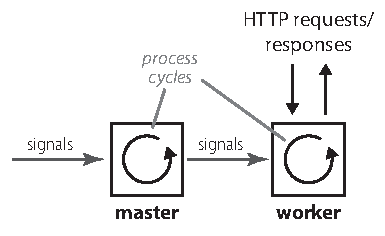
\includegraphics[scale=1]{images/nginx-overview.pdf}
	\caption{Overview of nginx process model.}
	\label{fig:nginx-overview}
\end{wrapfigure}

After initialization both processes run in a so called \textbf{process cycle}. That is an infinite loop with the process waiting to be activated from suspension by external events. For the master process these are signals send to the process which might indicate requests for shutdown, configuration reload or previously initiated timed events.

Design of the worker process had as key principle "to be as non-blocking as possible" \cite{aosa}. This is done by relying heavily on asynchronous operations being implemented through "modularity, event notifications, extensive use of callback functions and fine-tuned timers" \cite{aosa}. It also makes the process cycle of the worker process the "most complicated part of \textit{nginx}" \cite{aosa}.

Processing of requests is outsourced from the \textit{nginx} core routines to a number of dedicated modules. These modules hook into a processing pipeline forming a \textbf{chain of modules}. When a request receives, it is passed through the pipeline with every module doing the relevant work \cite{aosa}. Functionality of modules includes handling a specific protocol (e.g. \gls{http}), modifying content, filtering, handling special variables or load balancing. It is also possible to develop and integrate custom modules.

An \gls{http} request runs through a number of processing phases with dedicated \textbf{phase handlers}. These process a request and generate an appropriate response, send the header and send the body. Generation of content is done by \textbf{content handlers}. Out-of-the-box there exist several default handlers for index views or simple static files. The result of this handlers is passed to \textbf{filters} performing outbound content modifications. Filters form a separate processing pipeline, passing results among themselves until the final filter is called. Functionality of filters includes amongst others generation of header data, charset modification and gzip compression. \cite{aosa}

\subsection{Event-driven Architecture}

Another task of modules in the \textit{nginx} architecture is to implement functionality specific to a certain \gls{os}. One of this specifically designed tasks is the integration of an event module. Consistent and strict usage of the event-driven architecture is the fundamental point of \textit{nginx}.

This is accomplished by using asynchronous, i.e. non-blocking, i/o-functions of the operating system. Handling of returning events is done through an event module provided by the \gls{os}. For this project Linux's \textit{epoll}\footnote{\url{http://linux.die.net/man/4/epoll}} module is used. \textit{epoll} handles events on file descriptors. Therefore also network related and custom events can be handled, because in Linux everything is a file descriptor\footnote{Linus Torvalds, "The everything-is-a-file principle": \url{http://yarchive.net/comp/linux/everything_is_file.html} (as of 12/2012)} (or process).

Events are queued and dequeued in the worker process cycle. The total workload for processing a request is split into multiple chunks, each handled when necessary operations of the \gls{os} returned.

\begin{figure}[H]
	\centering
	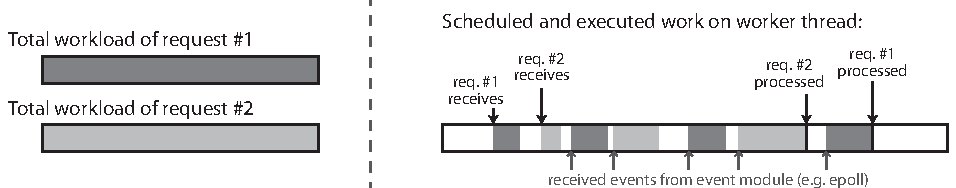
\includegraphics[scale=1]{images/nginx-event-proc.pdf}
	\caption{Processing model of worker threads.}
	\label{fig:nginx-event-proc}
\end{figure}

This leads to a responsive nginx worker thread which "can handle many thousands of concurrent connections and requests per second" (on a decent server system) \cite{aosa}.

\section{Configuration and Building}
\label{sec:nginx-config}

After this general overview of \textit{nginx}'s architecture and underlying concepts, the next section focuses on practical implications of bringing \textit{nginx} to a \textit{MicroBlaze} system.

\subsection{Extending the Configuration System}

The build process of \textit{nginx} can be configured with a number of parameters and constants to add or remove optional modules. The inclusion of modules can be configured with command line arguments to the configuration tool, but many of the parameters can not be set externally.

The values of these parameters are determined by a custom "auto configuration" tool. This tool writes small c programs to a temporary file, compiles them using the configured compiler and reads back the results. By this process \textit{nginx} adjusts its own build process to the features and properties of the current system. This configuration process is not working for cross-compiling \textit{nginx} for another target system. Therefore the configuration process needed to be extended to allow input of required configuration parameters into the build process from an external source.

The implemented solution is based on a suggested patch by Daniele Salvatore Albano\footnote{\textit{Cross compilation support for nginx}, Daniele Salvatore Albano, 01/03/2011 \url{http://web.archiveorange.com/archive/v/Tuw7Ryz8rztiNaIFfqCg}}, but incorporates more parameters and is streamlined to the process of cross-compiling the Linux kernel. Cross-compiling can be enabled by setting the environment variable "\texttt{CROSS\_COMPILE}" to the suitable compiler tool chain prefix. For the \textit{MicroBlaze} tool chain this is "\texttt{microblaze-unknown-linux-gnu-}".

Parameters that are covered by this modification to the configuration system include endianness (\texttt{with-endian}), the size of primitive data types (\texttt{with-int}, \texttt{with-long}, etc.) and the maximum error number, to be used for custom error types (\texttt{with-sys-nerr}).

Value for these introduced parameters can be determined through a small test program executed on the \gls{soc} (see appendix \ref{sec:nginx-env-eval}). This leads to the following values:

\begin{verbatim}
    --with-endian=big \
    --with-sys-nerr=132 \
    --with-int=4 \
    --with-long=4 \
    --with-long-long=8 \
    --with-ptr-size=4 \
    --with-sig-atomic-t=4 \
    --with-size-t=4 \
    --with-off-t=4 \
    --with-time-t=4
\end{verbatim}

\subsection{Modules}

\textit{nginx} consists of a number of (optional) modules. These modules can be in- or excluded from the build using parameters to the configuration tool. Objective of the \textit{nginx} build for the MicroBlaze system was a small binary with just the necessary parts included. There for the following modules were excluded:

\begin{verbatim}
    --without-http_rewrite_module \
    --without-http_gzip_module \
    --without-http_charset_module \
    --without-http_ssi_module \
    --without-http_userid_module \
    --without-http_access_module \
    --without-http_auth_basic_module \
    --without-http_autoindex_module \
    --without-http_status_module \
    --without-http_geo_module \
    --without-http_map_module \
    --without-http_split_clients_module \
    --without-http_referer_module \
    --without-http_proxy_module \
    --without-http_fastcgi_module \
    --without-http_uwsgi_module \
    --without-http_scgi_module \
    --without-http_memcached_module \
    --without-http_limit_conn_module \
    --without-http_limit_req_module \
    --without-http_empty_gif_module \
    --without-http_browser_module \
    --without-http_upstream_ip_hash_module \
    --without-http_upstream_least_conn_module \
    --without-http_upstream_keepalive_module \
    --without-http-cache \
    --without-pcre \
    --without-select_module \
    --without-poll_module
\end{verbatim}

Some of these modules could be included in the build, if necessary, but the modules \texttt{http\_rewrite\_module} and \texttt{http\_gzip\_module} require external libraries which are not present on the MicroBlaze system and therefore would not work.

\subsection{Compiler Configuration}

Besides the configuration for \textit{nginx} itself, the compiler needs to be configured for the target MicroBlaze system. When building the Linux kernel, the compiler configuration is set by the configuration of the kernel during the build process. \textit{nginx} does not have this functionality in its configuration system, but comes with a parameter (\texttt{--with-cc-opt=...}) to pass custom parameters to the compiler.

Through this configuration setting, the gcc cross-compiler needs to be configured for the feature set of the MicroBlaze system. For the presented MicroBlaze \gls{soc}, the required parameters are

\texttt{-mxl-multiply-high -mno-xl-soft-mul -mno-xl-soft-div} $\hookleftarrow$ \\
\texttt{-mxl-barrel-shift -mxl-pattern-compare -mcpu=v8.30.a}

Additionally the path to the standard libraries on the system needs to be set through the \texttt{--sysroot} parameter. These libraries are part of the tool chain for \textit{MicroBlaze} systems provided by \textit{Xilinx}. 

By specifying the \texttt{----static} parameter all referenced libraries are build into the resulting binary. Therefore the binary has less dependencies to be executed.

Combining it all together the value of the \texttt{--with-cc-opt} parameter needs to be set to something like the following: 

\texttt{--with-cc-opt="-mxl-multiply-high -mno-xl-soft-mul -mno-xl-soft-div} $ \hookleftarrow$ \\
\texttt{-mxl-barrel-shift -mxl-pattern-compare -mcpu=v8.30.a ----static} $ \hookleftarrow$ \\
\texttt{----sysroot=/home/peschuster/project/microblaze-unknown-linux-gnu/} $ \hookleftarrow$ \\
\texttt{microblaze-unknown-linux-gnu/sys-root"}

\subsection{Memory Leaks}

One problem that arose during tests were memory leaks. It turned out that \textit{nginx} allocated about 4053.2 Bytes of memory for each request. Assuming available memory of about 200 MB, \textit{nginx} crashed the complete system after approximately 50,500 requests in total. of course, this is an unacceptable behavior for a (web) server system.

\begin{figure}[H]
\begin{minipage}{0.4\textwidth}
\begin{tabular}{|r|r|r|}
    \hline
     \textbf{requests} & \textbf{master / KB} & \textbf{worker / KB} \\
    \hline
    0     & 3064  & 3204 \\
    1000  & 3064  & 7296 \\
    2000  & 3064  & 11256 \\
    3000  & 3064  & 15348 \\
    4000  & 3064  & 19440 \\
    5000  & 3064  & 23404 \\
    6000  & 3064  & 27496 \\
    7000  & 3064  & 31588 \\
    8000  & 3064  & 35552 \\
    9000  & 3064  & 39644 \\
    10000 & 3064  & 43736 \\
    \hline
    \end{tabular}
\end{minipage}
\begin{minipage}{0.60\textwidth}
	\centering
	\begin{tikzpicture}
		\begin{axis}[width=\textwidth,height=7cm,
			xlabel={requests},
			ylabel={memory / KB},
			xmin=0,
			ymin=0,
			xmax=10000,
			extra y ticks={3064},
			%extra y tick label style={/pgf/number format/1000 sep=},
			extra y tick style={grid=major},
			extra x tick style={grid=major},
			y tick label style={/pgf/number format/1000 sep=},
			legend pos = north west]
			\addplot table[x index=0, y index=1] {graphdata/nginx-mem.csv};
			\addlegendentry{master process}
			\addplot table[x index=0, y index=2] {graphdata/nginx-mem.csv};
			\addlegendentry{worker process}
		\end{axis}
	\end{tikzpicture}
\end{minipage}
  \caption{Memory consumption of nginx processes over total requests.}
  \label{fig:nginx-mem}
\end{figure}

\subsubsection{Investigations}

The described behavior of \textit{nginx} could not be replicated on a standard x86 server system running \textit{Ubuntu Linux 12.04}. That means \textit{nginx} in general should work correct, using just as much memory as required and releasing unused memory to the \gls{os}. However, on the \textit{MicroBlaze} system this does not work properly.

With activated \texttt{debug} log. \textit{nginx} writes some information about inner workings to the error log. The debug log can be activated with the following option in the configuration file:

\begin{verbatim}
error_log  logs/error.log  debug;
\end{verbatim}

There must be only one \texttt{error\_log} line in the \textit{nginx} configuration file, but the option specifying the severity level is inclusive for all lower levels.

The following table shows all memory related debug messages as found in the error log for a single request to a static file on the \textit{MicroBlaze} system running a \textit{nginx} instance, which is configured as described in the previous section (\ref{sec:nginx-config}):

\begin{table}[H]
\centering
\begin{tabular}{|l|l|r|r|}
    \hline
     \textbf{Log entry} & \textbf{ptr} & \textbf{allocated} & \textbf{freed} \\
    \hline \hline
\texttt{*1 malloc: 10080890:644} & 10080890 & 644 &  \\ \hline
\texttt{*1 malloc: 10080B18:1024} & 10080B18 & 1024 &  \\ \hline
\texttt{*1 posix\_memalign: 1007B5B0:4096 @16} & 1007B5B0 & 4096 &  \\ \hline \hline
\texttt{*1 free: 1007B5B0, unused: 2079} & 1007B5B0 & & 4096 \\ \hline
\texttt{*1 free: 10080890} & 10080890 & & 644 \\ \hline
\texttt{*1 free: 10080B18} & 10080B18 & & 1024 \\ \hline
\end{tabular}
\caption{Memory management related debug messages of a single request.}
\label{tab:debug_mem}
\end{table}

All pointers to allocated memory for one request are passed to the \texttt{free(..)} function of the \textit{C Standard Library} (\textit{libc}) and therefore should be released to the system. But performance and stress tests on the system proved a different behavior: The \textit{nginx} worker process consumes more memory for each request with a linear relation to the number of requests (see \ref{fig:nginx-mem}).

Therefore the error causing this misbehavior probably is not located in \textit{nginx} itself, but in the underlying system layers. This would mean that memory management of the Linux kernel or \textit{libc} port to the \textit{MicroBlaze} architecture are broken, in the described respect. This is a strong allegation, especially because fully analyzing the problem on this wide dimensions was beyond the scope of this bachelor thesis. But there are a view points promoting this theory which should be considered:

There is an answer by \textit{Xilinx} support (\textit{AR \#12421}) stating that memory management (especially the function \textit{free(..)}) is "very system-specific" and not fully implemented/supported for \textit{MicroBlaze} processors \cite{mbfree}. The answer was published on 09/09/2010 and is explicitly only valid for versions of the \textit{MicroBlaze} processors without a hardware memory management unit. Therefore it should not apply to the used version of the \textit{MicroBlaze} processor and \textit{C Standard Library}, but it shows that these memory management functions were added to the toolchain and supporting environment only recently and might not be as stable as other parts.

Another point benefiting this theory is the unusual way \textit{nginx} deals with memory. Memory management is done by \textit{nginx}'s pool allocator. This could be seen as an abstraction to the memory allocation mechanisms provided by the \gls{os}. When a module/sub-routine/function requires dynamically allocated memory, it requests it from the \textit{nginx} pool allocator, which itself requests a larger chunk of memory (called "pool") from the \gls{os} and distributes small blocks of the pool on requests from other parts of \textit{nginx}. When no blocks of a pool are used anymore, it is returned to the \gls{os}. \textit{nginx} uses this design to minimize system calls and reduce expensive requests for memory allocation by the hardware memory management unit \cite{aosa}. Another consequence of this design is that \textit{nginx} does not reuse once allocated memory, but just allocates new memory blocks when required and releasing them to the system upon finished operations. This is by design and beneficial for speed and efficiency, but comes in unfavorable, when the memory management of the system (\gls{os} and processor) might not work properly.

\subsubsection{A First Workaround}

It was not possible to fix the root cause of the memory leaks during this bachelor thesis. To circumvent the described arising problems, another solution needed to be found to be able to use the system and conduct extensive performance tests.

A workaround to circumvent complete system crashes during tests due to exhausted memory is to restart the \textit{nginx} worker process on low remaining system memory.

This can be accomplished by sending the \texttt{HUB} signal to the \textit{nginx} master process using the \texttt{kill} command of \textit{Unix} systems\footnote{\url{http://unixhelp.ed.ac.uk/CGI/man-cgi?kill}}. The \texttt{HUB} signal tells \textit{nginx} to reload the current configuration, resulting in spinning up new worker processes and gracefully shutting down the previous ones. This differs from complete restarts of \textit{nginx} in the way that no incoming requests are lost during the restart process\footnote{\url{http://wiki.nginx.org/CommandLine} (as of 12/2012)}.

The process id of the master process on the system under test is always stored in the file \texttt{/usr/local/nginx/logs/nginx.pid}. Therefore the complete command for restarting the \textit{nginx} worker process can be constructed as follows:

\begin{verbatim}
kill -HUP $( cat /usr/local/nginx/logs/nginx.pid )
\end{verbatim}

Information about currently allocated and free memory can be displayed using tools like \textit{top}\footnote{\url{http://www.busybox.net/downloads/BusyBox.html\#top}}, which provide "a view of process activity in real time" \cite{busybox}. \textit{top} internally aggregates information from multiple (virtual) file handles like e.g. \texttt{/proc/meminfo} for information about memory.

\subsubsection{An Integrated Solution}

This workaround works well, but requires manual actions by a user and is therefore ignorant for automation which is a key part of extensive performance tests.

An idea for an extended solution was to shift checking for low remaining memory to the \textit{nginx} master process.

After configuring and building up the system, including the start of worker processes, the master process returns to a standby mode, waiting for external signals (like the previously described \texttt{HUB} signal). This is implemented using the default \textit{C Standard Library} signal implementation, mainly \texttt{sigsuspend}\footnote{\url{http://www.gnu.org/software/libc/manual/html\_node/Sigsuspend.html}}, inside of the \texttt{ngx\_master\_process\_cycle(..)} function (in the file \texttt{ngx\_worker\_cycle.c}).

A developed patch to check memory consumption of the system and initiate worker process restarts hooks in at this point inside of the master process. 

The patch consists of three major parts:

\begin{enumerate}

\item Starting a timer, to awake the master process every second from suspension. This is implemented using the Linux command \texttt{setitimer}\footnote{\url{http://linux.about.com/library/cmd/blcmdl2\_setitimer.htm}} in \texttt{ITIMER\_REAL} mode to send a \texttt{SIGALRM} signal to the hosting (i.e. \textit{nginx} master) process.

\item A signal handler for dealing with the \texttt{SIGALRM} signal, to check the remaining system memory and trigger a restart of the worker processes, if necessary.

\item A function reading the file handle \texttt{/proc/meminfo}, parsing out the required information about free system memory and comparing it with a configured threshold value. This is implemented in the new file \texttt{ngx\_process\_memguard.c}.
\end{enumerate}

Usage of the newly implemented functionality needs to be activated upon build configuration by providing the parameter \texttt{----with-min-free-mem=[value]}. \texttt{[value]} is the threshold value in bytes which is compared to the free system memory to decide on a required restart of worker processes. During tests of the system this value was set to "\texttt{51200}" (kilobytes).

The complete patch is included in the appendix of this report (see \ref{appendix:memguard}) or can be found in the master branch of the \textit{nginx} fork at \url{https://github.com/peschuster/nginx}.

\section{Compilation and Installation}

After configuration the \textit{nginx} binary file is compiled using "\texttt{make -f objs/Makefile}". The resulting image file has a size of about 1.8 MB.

Installation into the target directory is initiated executing the command "\texttt{make install DESTDIR=<dir>}". "\texttt{<dir>}" needs to be replaced with the path to the target directory. In the used environment during this project this is the directory of the target file system "\texttt{/home/peschuster/project/customfs/complete}".

Executing the described \texttt{install} command creates the required directory structure with default configuration files and copies the image file.

\section{Runtime Configuration}

Configuration of an \textit{nginx} installation is stored in the \texttt{conf/} directory relative to the \textit{nginx} root. For this project and conducted performance tests, there was no need to change the default configuration (\texttt{nginx.conf}), which is loaded at application start up when no other options are specified.

\section{Interfaces to the Operating System}
\label{sec:nginx-os-if}

This section briefly describes interactions between \textit{nginx} and the underlying \gls{os} to deal with HTTP requests and responses.

User applications can interact with the network stack implemented in the Linux kernel using the \textbf{socket}\footnote{\url{http://linux.die.net/man/7/socket}} interface.

nginx master process opens sockets using the \texttt{socket(..)} command and binds them to configured addresses using \texttt{bind(..)}. By default this is port \texttt{80} on all IP addresses (\texttt{0.0.0.0:80}). Last step during initialization is a call to \texttt{listen(..)} to indicate that \textit{nginx} is ready for accepting incoming connections.

nginx worker process initializes the core event module, which itself registers the callback \texttt{ngx\_event\_accept(..)} for incoming connections. Inside of \texttt{ngx\_event\_accept} the system call \texttt{accept(..)} is made.

Responses for requests to static files are written to the socket buffer using the two functions \texttt{writev} (for HTTP header data) and \texttt{sendfile} for content of the actual static file. This leads to atleast two TCP packets, always (see introduction to performance tests: \ref{subsec:mtu}).

Data is read from sockets using \texttt{recv(..)} which is called on parsing the HTTP request header, but also on demand in several phases of an \textit{nginx} worker thread.
\chapter{Performance-Analysis}

Before going into performance tests, it is required to understand some fundamentals about network communication and the anatomy of a \gls{http} request.

\section{Introduction}

"To reduce their design complexity, most networks are organized as a \textbf{stack of layers or levels}, each one built upon the one below it" \cite{kn1}[sec. 1.3.1]. The same holds true for the protocol stack driving the "internet". There exist various models for naming and describing the different layers. In context of the internet usually the "TCP/IP Reference Model" is used \cite{kn1}. This model describes five independent layers, each build upon the next underlying layer. 

Real communication between two systems, i.e. exchange of data, always happens on the lowest layer (the "Physical Layer"). But from a logical point of view, communication happens on each layer between the two systems. Therefore each layer might add a header in front of the data, specifying meta information for its counterpart on the other system. Headers of layers above the current layer are treated as plain data, just as the actual message (see figure \ref{fig:header-layers}).

%\begin{wrapfigure}{r}{.45\textwidth}
\begin{figure}[H]
	\centering
	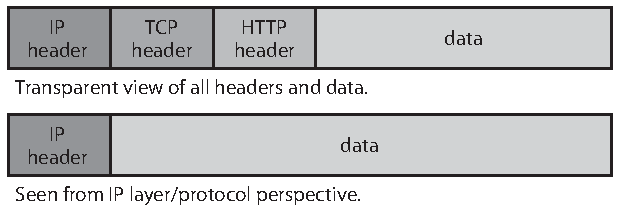
\includegraphics[scale=1]{images/protocol-headers.pdf}
	\caption{Header data for multiple protocol layers.}
	\label{fig:header-layers}
\end{figure}
%\end{wrapfigure}

Figure \ref{fig:net-layers} shows the five layers of the TCP/IP model with corresponding communication protocol and module implementing the protocol on the developed test system. When constructing performance tests this needs to be taken into account to determine for a single parameter which parts of the system are involved and might limit further improvements.

%\begin{wrapfigure}{r}{.5\textwidth}
\begin{figure}[H]
	\centering
	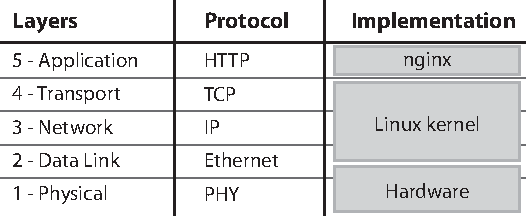
\includegraphics[scale=1]{images/network-layers.pdf}
	\caption{Layers of the network stack with reference to implementing modules.}
	\label{fig:net-layers}
\end{figure}
%\end{wrapfigure}

\subsection{Maximal Transfer Unit (MTU)}
\label{subsec:mtu}

The \gls{mtu} is the maximum size of a single unit transferred over the network in bytes. It is a parameter set for a complete network (sender, receiver, intermediate stations), specifying and limiting its capacity to a robust and reliable usage level. On differing \gls{mtu} values for connected stations the lowest takes effect. In Ethernet networks the \gls{mtu} is usually set to 1500 bytes \cite{kn1}. This includes only the data as received by the Ethernet layer. Header data of  the Ethernet protocol does not count into this size limit. When messages (including header data of upper layers) exceed the \gls{mtu} size, they are split up into multiple packets. In practice this means that for transmitting a single HTTP message (i.e. request or response) two or more \gls{tcp} messages might be required.

\subsection{Transmission Control Protocol (TCP)}

Although \gls{http} is not fixed to be used only with \gls{tcp}; \gls{http} on top of \gls{tcp} on top of \gls{ip} is the most dominant usage combination. This is, because \gls{tcp} provides reliable communication on top of unreliable networks \cite{tcp}. \gls{tcp} accomplishes this by setting up and maintaining a connection. Therefore sending data over TCP consists of three steps: establishing a connection, sending the actual message, closing the connection. To guarantee arrival of sent data, \gls{tcp} works with a handshake protocol between both involved parties. Maintaining a connection is the price to be paid for a reliable communication channel between two systems. But it also allows sending more than one messages using an already established connection. This comes in handy, when a message size exceed the \gls{mtu} or multiple \gls{http} requests are send to a server (used in persistent HTTP connections, also called "HTTP keep-alive" \cite{http}).

\gls{ip} introduced so called IP addresses as identifiers for single systems. \gls{tcp} extends this model by port numbers. An application providing services to other system (i.e. a server) uses one single port, but client applications need to open separate ports for each \gls{tcp} connection. This is required, because \gls{tcp} connections are identified by the four parts "server address", "server port", "client address" and "client port" \cite{tcp}. The TCP header contains two 16 bit fields for source and destination port \cite{kn1}. This leads to a maximum of $2^{16} = 65,536$ concurrently used (open) \gls{tcp} connections on a single client system.

\section{Measuring Web Server Performance}

Network performance is often measured as throughput in bits per second. While this gives a great insight in the capabilities of the network, there is no indication as to how many users can be served concurrently by a web server running on the system under test. To gain insights in this performance parameter, dedicated tests on \gls{http} level need to be performed.

A simple method for measuring request throughput is to "send requests to the server at a fixed rate and to measure the rate at which replies arrive" \cite{httperf}. By monotonically increasing the request rate, the server becomes saturate  at a certain point. This becomes visible in leveling off reply rates and shows that the server operates at full capacity. \cite{httperf}

\subsection{Tools}

\subsubsection{httperf}

\textit{httperf}\footnote{\url{http://www.hpl.hp.com/research/linux/httperf/}} is a tool developed at Hewlett-Packard by David Mosberger and Tai Jin to specifically measure web server performance \cite{httperf}.

\textit{httperf} has three relevant command line arguments for performing the desired performance tests: \texttt{rate}, \texttt{num-conns} and \texttt{num-calls}.

The \texttt{rate} parameter specifies the rate at which connections are created per second. \texttt{num-conns} specifies the total number of connections to be created during one test run. \texttt{num-calls} specifies the number of requests made over a single TCP connection before it is closed.

When executing \textit{httperf} a warning might be displayed:

\texttt{warning: open file limit > FD\_SETSIZE; limiting max. \# of open files to FD\_SETSIZE}

What it basically means is that the current process reached the limit of concurrently allowed open file descriptors. This is a per process limit enforced by the \gls{os}. \textit{httperf} is using the \textit{select}\footnote{"\texttt{select}" is an event library provided by the Linux kernel.} module for dealing with network tasks and creates a new file descriptor for every TCP connection. Therefore the limit on open file descriptors limits the number of TCP connections by \textit{httperf} and therefore might influence conducted performance tests.

To circumvent this issue limits on the current system need to be increased and \textit{httperf} re-compiled. This includes three steps\footnote{The described solution to the FD\_SETSIZE problem was taken from Guillaume Maury: \url{http://gom-jabbar.org/articles/2009/02/04/httperf-and-file-descriptors}.}:

\begin{enumerate}
\item The following line needs to be inserted (or updated) in \texttt{/etc/security/limits.conf}: "\texttt{* hard nofile 65535}". This increases the hard limit of open file descriptors for all users.

\item The value of the pre-compiler constant "\texttt{\_\_FD\_SET\_SIZE} needs to be increased to \texttt{65535}. It is defined in "\texttt{/usr/include/bits/typesizes.h}". (Note: This file might be located in another sub-directory, e.g. "\texttt{/usr/include/x86\_64-linux-gnu/bits/typesizes.h}".)

\item httperf needs to be re-compiled from source:\\
 \\
\texttt{wget} \url{ftp://ftp.hpl.hp.com/pub/httperf/httperf-0.9.0.tar.gz}\\
\texttt{tar xvzf httperf-0.9.0.tar.gz \&\& cd httperf-0.9.0\\
./configure \&\& make\\
sudo make install}
\end{enumerate}

A useful helper for automating test runs with increasing connection rate is \textit{autobench}\footnote{\url{http://www.xenoclast.org/autobench/}}. It is a Perl script acting as a wrapper around \textit{httperf} written by Julian Midgley.

\subsubsection{Custom Scripts}

In addition to accurate engineered test cases using \textit{httperf}, custom scripts were used to simply generate load on the server. A small Windows console application written in \texttt{C\#}, utilizing the \textit{Task Parallel Library}\footnote{\url{http://msdn.microsoft.com/de-de/library/vstudio/dd460717.aspx}} turned out to be the most efficient one with best performance characteristics.

It is also included in the appendix of this report (see \ref{appendix:csharp-load}).

\subsubsection{Wireshark}

\textit{Wireshark}\footnote{\url{http://www.wireshark.org}} is a network protocol analysis software, which captures all traffic going through a network interface. It especially helps in analyzing and inspecting captured data through deep knowledge of all common protocols.

It was used in this project for debugging initial problems with the network stack and low-level analysis of performance  test parameters.


\section{Tests}

The tests were conducted using \textit{httperf} on a virtual machine running \textit{Ubuntu Linux 12.04}. To proof that the limiting factor during the tests is not this client machine, but the system under test, all tests were also performed against a \textit{Microsoft IIS 7.5} web server instance on top of a \textit{Microsoft Windows 7 Professional} operating system running on a bare metal machine with an \textit{AMD Phenom II X4 965} processor at 3.40 GHz.

According to the \textit{HTTP Archive}\footnote{\url{http://httparchive.org/interesting.php\#responsesizes} (as of Dec. 15th 2012)} an average HTML page has a size of about 6 kB. Other content types, like images, stylesheets and script files vary on average between 5 kB and 21 kB. Therefore tests were performed using static files with two sizes: one file having exactly 10 kB (10.240 bytes) from now on referred to as "10K.html" and one very minimal HTML page having just 354 bytes ("index.html"). The major difference between these two files from a "network perspective" is that the small file can be transmitted in two TCP packets (one for the HTTP header and one for the actual data, see section \ref{sec:nginx-os-if}), whereas the 10 KB file needs to be split up in 9 TCP packets due to the default \gls{mtu} size of 1500 bytes.

The following figure (\ref{fig:initial-req}) shows request and response rates two both files with an increasing connection rate (20 conn./s to 120 conn./s, step size: 10). On each connection three HTTP requests were made to the respective file. On every connection rate level 3.000 connections were opened to obtain reliable results.

\begin{figure}[H]
	\centering
	\begin{tikzpicture}
		\begin{axis}[width=\textwidth,height=7cm,
			xlabel={demanded request rate (per second)},
			ylabel={per second},
			extra y tick style={grid=major},
			extra x tick style={grid=major},
			y tick label style={/pgf/number format/1000 sep=},
			ymajorgrids=true,
			legend pos = south east]
			\addplot table[x index=0, y index=1] {graphdata/perf-initial2.csv};
			\addlegendentry{request rate (index.html)}
			\addplot table[x index=0, y index=8] {graphdata/perf-initial2.csv};
			\addlegendentry{reponse rate (index.html)}
			\addplot table[x index=0, y index=2] {graphdata/perf-initial2.csv};
			\addlegendentry{request rate (10K.html)}
			\addplot table[x index=0, y index=9] {graphdata/perf-initial2.csv};
			\addlegendentry{reponse rate (10K.html)}
		\end{axis}
	\end{tikzpicture}
  \caption{Request and response rates for two static files (\texttt{10K.html} and \texttt{index.html}).}
  \label{fig:initial-req}
\end{figure}

The difference between request and response rate origins in failed requests. The following figure shows the corresponding error rate which increases with over-saturating the system.

\begin{figure}[H]
	\centering
	\begin{tikzpicture}
		\begin{axis}[width=\textwidth,height=6cm,
			xlabel={demanded request rate (per second)},
			ylabel={error rate (\%)},
			extra y tick style={grid=major},
			extra x tick style={grid=major},
			y tick label style={/pgf/number format/1000 sep=},
			minor tick style={very thin, gray},
			minor y tick num=3,
			ymajorgrids=true,
			legend pos = north west]
			\addplot table[x index=0, y index=15] {graphdata/perf-initial2.csv};
			\addlegendentry{index.html}
			\addplot table[x index=0, y index=16] {graphdata/perf-initial2.csv};
			\addlegendentry{10K.html}
		\end{axis}
	\end{tikzpicture}
  \caption{Error rate (failed requests) for two static files (\texttt{10K.html} and \texttt{index.html}).}
  \label{fig:initial-req-errors}
\end{figure}

The response \textbf{rate} decreases only slowly with growing saturation, but the average response \textbf{time} increases from  5 ms to about 500-650 ms:

\begin{figure}[H]
	\centering
	\begin{tikzpicture}
		\begin{axis}[width=\textwidth,height=6cm,
			xlabel={demanded request rate (per second)},
			ylabel={response time / ms},
			extra y tick style={grid=major},
			extra x tick style={grid=major},
			y tick label style={/pgf/number format/1000 sep=},
			minor tick style={very thin, gray},
			minor y tick num=3,
			ymajorgrids=true,
			legend pos = south east]
			\addplot table[x index=0, y index=10] {graphdata/perf-initial2.csv};
			\addlegendentry{index.html}
			\addplot table[x index=0, y index=11] {graphdata/perf-initial2.csv};
			\addlegendentry{10K.html}
		\end{axis}
	\end{tikzpicture}
  \caption{Response time for two static files (\texttt{10K.html} and \texttt{index.html}).}
  \label{fig:initial-req-time}
\end{figure}

\begin{wrapfigure}[16]{r}{.5\textwidth}
	\centering
	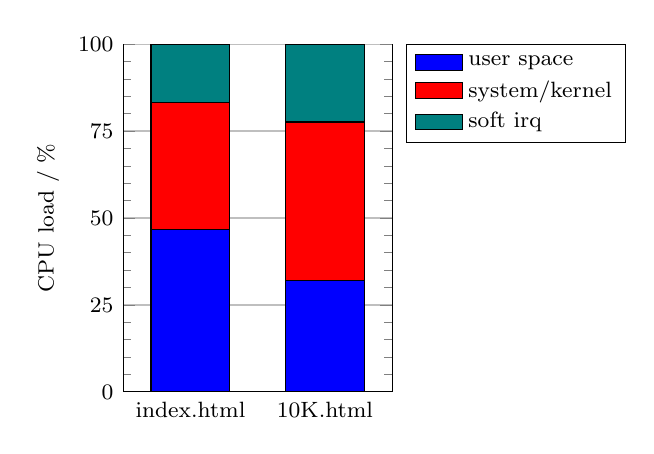
\begin{tikzpicture}
		\begin{axis}[ybar stacked,
			legend style={at={(1.05,1.0)},anchor=north west},
			xtick={0,1},
			axis x line*=bottom,
			tick label style={font=\footnotesize},
			legend style={font=\footnotesize},
			label style={font=\footnotesize},
			ytick={0,25,50,75,100},
			width=5cm,
			height=6cm,
			bar width=10mm,
			ylabel={CPU load / \%},
			xticklabels={index.html, 10K.html},
			ymajorgrids=true,
			minor tick style={very thin, gray},
			minor y tick num=4,
			ymin=0,
			ymax=100,
			area legend,
			legend cell align=left,
			enlarge x limits=0.5]
			\addplot[fill=blue] coordinates % usr
			{(0,46.6) (1,32.1)};
			\addplot[fill=red] coordinates % sys
			{(0,36.5) (1,45.5)};
			\addplot[fill=teal] coordinates % sirq
			{(0,16.7) (1,22.3)};
			\legend{user space,system/kernel,soft irq}
		\end{axis}
	\end{tikzpicture}
	\caption{CPU load distribution for different request types.}
  \label{fig:initial-req-cpu}
\end{wrapfigure}

The difference in request and response rates the system can handle is also visible in \textbf{CPU utilization}. Main responsibility of \textit{nginx} for serving requests is to handle the HTTP part. This includes parsing the request header, generating responses and delivering static files. The \gls{os} on the other hand does the "translation" to and from \gls{tcp} and handles all lower layers (see also figure \ref{fig:net-layers}). An increased payload size of single responses entails therefore a shift in processing time from \textit{nginx} ("user space") to the operations inside the Linux kernel.

The \textbf{network throughput} of both tests follows naturally the trend of response rates. For the test requesting the "index.html" file, the shown throughput is very low, because \textit{httperf} calculates the average throughput as $\cfrac{\text{[size]} \cdot \text{[total repsonses]}}{\text{[test time]}}$.
\vspace{1cm}

\begin{figure}[H]
	\centering
	\begin{tikzpicture}
		\begin{axis}[width=\textwidth,height=6cm,
			xlabel={demanded request rate (per second)},
			ylabel={KB / s},
			extra y tick style={grid=major},
			extra x tick style={grid=major},
			y tick label style={/pgf/number format/1000 sep=},
			minor tick style={very thin, gray},
			minor y tick num=3,
			ymajorgrids=true,
			legend pos = north west]
			\addplot table[x index=0, y index=13] {graphdata/perf-initial2.csv};
			\addlegendentry{index.html}
			\addplot table[x index=0, y index=14] {graphdata/perf-initial2.csv};
			\addlegendentry{10K.html}
		\end{axis}
	\end{tikzpicture}
  \caption{Throughput for two static files (\texttt{10K.html} and \texttt{index.html}).}
  \label{fig:initial-req-io}
\end{figure}

\clearpage
\subsection{Network throughput}

To test the maximal network throughput the server can provide, a test needs to be designed focusing just this parameter to prevent other parts of the system under test to get into the way. A constant high exchange of TCP packets can be achieved by transferring single large files over the network. Therefore a large binary (movie) file with a payload size of 33.4 MB was used for throughput tests.

The following figure (\ref{fig:tcp-io-perf}) shows the network throughput for requests to this file with an increasing connection rate and two requests per connection. The system under test goes into saturation at about 61 Megabits/sec. The figure also shows the total CPU utilization of the tested system.

\begin{figure}[H]
	\centering
	\begin{tikzpicture}
		\begin{axis}[width=\textwidth,height=6cm,
			xlabel={connection rate},
			ylabel={$10^6$ bits/s},
			axis  y  line*=left,
			extra y tick style={grid=major},
			extra x tick style={grid=major},
			y tick label style={/pgf/number format/1000 sep=},
			minor tick style={very thin, gray},
			minor y tick num=3,
			ymajorgrids=true,
			legend style = {at={(0.125,-.1)}, anchor=north}]
			\addplot[color=blue,mark=o] table[x index=0, y index=13] {graphdata/tcp-io-perf.csv};
			\addlegendentry{network throughput}
		\end{axis}
		\begin{axis}[width=\textwidth,height=6cm,
			ylabel={percentage},
			axis  y  line*=right,
			axis  x  line=none,
			extra y tick style={grid=major},
			extra x tick style={grid=major},
			y tick label style={/pgf/number format/1000 sep=},
			minor tick style={very thin, gray},
			minor y tick num=3,
			%ymajorgrids=true,
			legend style = {at={(0.93,-.1)}, anchor=north}]
			\addplot[color=red,mark=x] table[x index=0, y index=9] {graphdata/tcp-io-perf.csv};
			\addlegendentry{cpu load}
		\end{axis}
	\end{tikzpicture}
  \caption{Network throughput and CPU load.}
  \label{fig:tcp-io-perf}
\end{figure}

The following figure (\ref{fig:tcp-io-perf-cpu}) shows the CPU utilization by time spent in the different types of the system. It shows that most time is spent in kernel space and handling interrupt requests by the network driver and sub system. nginx (user space) takes only very low CPU utilization and is not the limiting factor in this test.

%usr	%CPU spent by User space applications		
%sys	%CPU spent by the System (kernel mode)		
%nic	%CPU spent by Low priority user mode (nice)		
%Idle	%CPU which is available (idle)		
%io		%CPU spent by I/O waiting		
%irq	%CPU spent servicing interrupt requests		
%sirq	%CPU spent servicing soft irqs	

\begin{figure}[H]
	\centering
	\begin{tikzpicture}
		\begin{axis}[ybar stacked,width=\textwidth,height=6cm,
			xlabel={connection rate},
			ylabel={percentage},
			extra y tick style={grid=major},
			extra x tick style={grid=major},
			y tick label style={/pgf/number format/1000 sep=},
			minor tick style={very thin, gray},
			minor y tick num=3,
			ymajorgrids=true,
			bar width=10mm,
			area legend,
			legend columns=6,
			legend style = {at={(0.5,1.03)}, anchor=south}]
%			legend pos = south east]
			\addplot[fill=red] table[x index=0, y index=2] {graphdata/tcp-io-perf.csv};	%,mark=x
			\addlegendentry{user space  }
			\addplot[fill=blue] table[x index=0, y index=3] {graphdata/tcp-io-perf.csv};	%,mark=o
			\addlegendentry{system/kernel}
%			\addplot[color=magenta,mark=o] table[x index=0, y index=4] {graphdata/tcp-io-perf.csv};
%			\addlegendentry{low priority (nice)}
%			\addplot table[x index=0, y index=5] {graphdata/tcp-io-perf.csv};
%			\addlegendentry{idle}
%			\addplot[color=orange,mark=triangle] table[x index=0, y index=6] {graphdata/tcp-io-perf.csv};
%			\addlegendentry{io (waiting)}
%			\addplot[color=green,mark=|] table[x index=0, y index=7] {graphdata/tcp-io-perf.csv};
%			\addlegendentry{irq}
			\addplot[fill=teal] table[x index=0, y index=8] {graphdata/tcp-io-perf.csv};	%,mark=diamond
			\addlegendentry{soft irq}
		\end{axis}
	\end{tikzpicture}
  \caption{CPU utilization by category.}
  \label{fig:tcp-io-perf-cpu}
\end{figure}

To proof that obtained performance limits were not limits of the client executing the tests or the network infrastructure, the same test was executed against the "reference system" running an \textit{Microsoft IIS 7.5} web server. Figure \ref{fig:tcp-io-perf-iis} shows the results which outplays the results of the \textit{MicroBlaze} system by more than a factor of eight:

\begin{figure}[H]
	\centering
	\begin{tikzpicture}
		\begin{axis}[width=\textwidth,height=6cm,
			xlabel={connection rate},
			ylabel={$10^6$ bits/s},
			extra y tick style={grid=major},
			extra x tick style={grid=major},
			y tick label style={/pgf/number format/1000 sep=},
			minor tick style={very thin, gray},
			minor y tick num=3,
			ymajorgrids=true,
			legend pos = south east]
			\addplot table[x index=0, y index=15] {graphdata/tcp-io-perf.csv};
			\addlegendentry{network throughput}
		\end{axis}
	\end{tikzpicture}
  \caption{Network throughput of an AMD Phenom II X4 processor at 3.40 GHz running Microsoft IIS 7.5 on Windows 7.}
  \label{fig:tcp-io-perf-iis}
\end{figure}

\chapter{Overview of the Linux Network Stack}

\begin{wrapfigure}[20]{r}{.35\textwidth}
	\centering
	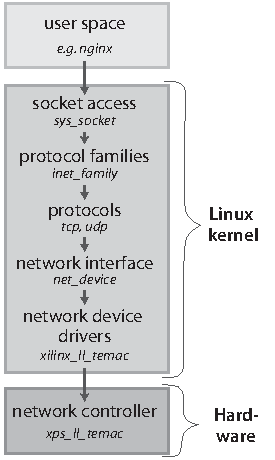
\includegraphics[scale=1]{images/net-stack.pdf}
	\caption{Linux network stack.}
	\label{fig:net-stack}
\end{wrapfigure}
The top most layer of the Linux network stack is the \textbf{system call interface} to create and operate on sockets \cite{netstackana}. The usage of this interface by \textit{nginx} is already described in section \ref{sec:nginx-os-if}. Its purpose is to multiplex networking calls by the user into the kernel \cite{netstackana}. Once a file descriptor was created using the socket interface, data can be exchanged with the network system through general operations on file descriptors like \textit{write} and \textit{read}, too. The socket interface is completely agnostic to different protocols or implementations by network devices and drivers. Its main underlying structure is "\texttt{struct sock}", containing all relevant information about a specific socket, like available functions and protocol specific state information.\footnote{\url{http://www.ecsl.cs.sunysb.edu/elibrary/linux/network/LinuxKernel.pdf}} Thereby also protocol and implementation specific functionality is bind to a socket using function pointers (defined in "\texttt{struct inet\_protosw}") \cite{netstackana}.

Whereas the more general data structure "\texttt{struct sock}" contains mainly meta information about a socket, the major structure for storing data is "\texttt{struct sk\_buff}". \textbf{\texttt{sk\_buff}} contains packet data and state information. It is used for to be sent, as well as for received packets almost through out all layers of the network stack. \cite{netstackana}

The gap between protocol handling and device drivers is bridged by the \textbf{network interface} (\textit{netif}) layer. This is a hardware device "agnostic interface layer" \cite{netstackana}. Its major purpose is to connect protocols to hardware devices. Information about devices is provided through "\texttt{struct net\_device}". On system start-up all available devices register themselves with a filled out "\texttt{net\_device}" structure. From there on they are know to the network interface layer.

The lowest layer of the network stack being part of the Linux kernel is formed by \textbf{device drivers}. These hook into the network interface layer and manage physical/hardware network controllers. For the implemented System on Chip this is the \texttt{xps\_ll\_temac} \gls{ip} core.

\begin{wrapfigure}[10]{r}{.23\textwidth}
	\centering
	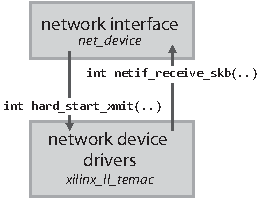
\includegraphics[scale=1]{images/netif-dev.pdf}
	\caption{\texttt{sk\_buff} exchange}
	\label{fig:netif-dev}
\end{wrapfigure}

Since introduction of the "New API" (\textit{NAPI}) for communication between device drivers processing packets and the network interface layer, most of the workload for received and to be sent packets is scheduled using software interrupt requests (also known as "\textit{soft irq}" or "\textit{sirq}").\footnote{\url{http://www.linuxfoundation.org/collaborate/workgroups/networking/napi} (as of 12/2012)} During performance tests described in the previous chapter this was visible through high CPU utilization of the \textit{sirq} category.

The network interface layer enqueues \texttt{sk\_buff} packets for transmission using the function \texttt{int hard\_start\_xmit(struct sk\_buff *skb, struct net\_device *dev)}. Usually a call to this function is protected with a \textit{lock} to protect it from being called multiple times simultaneously.\footnote{\url{http://lwn.net/Articles/120960/} (as of 12/2012)} The device driver pushes received packets to the upper layer using \texttt{int netif\_receive\_skb(struct sk\_buff *skb)}. \cite{netstackana}

\chapter{TCP Offload Engine}

\section{Overview}

\subsection{Benefits}

Conducted performance tests showed\footnote{see figures \ref{fig:initial-req-cpu} and \ref{fig:tcp-io-perf-cpu}} that much processing time is spend handling interrupt requests of the network sub system. Especially on TCP-heavy-requests this circumstance tuned out to be a bottleneck for a system with little processing power like the designed System on Chip.

Handling of TCP connections and processing messages is on the other hand a well defined and general problem that could be outsourced to an own "processor", leaving more processing power of the main system (\gls{cpu}) for other tasks. This is the approach of \textit{TCP Offload Engines} (TOE).
\\

\subsection{State of the Art}

Throughout recent years some attempts by hardware vendors developingBücher network interface cards were made to integrate support for \textit{TCP Offload Engines} into the Linux kernel (e.g. by \textit{Chelsio Communications}: \url{http://lwn.net/Articles/147289/}). However, maintainers\footnote{\url{http://lwn.net/Articles/148701/}} of the Linux network stack and the \textit{Linux Foundation}\footnote{\url{http://www.linuxfoundation.org/collaborate/workgroups/networking/toe}} have a strong opinion against integrating drivers and support through out the network stack for these hardware devices.

This is partially based on reservations about quality standards and the lack of possible benefits, but includes also arguments of a more general nature. A \textit{TOE} would "short out much of the Linux networking code" and therefore "cut out little features like \textit{netfilter}, traffic control, and more" \cite{linux-toe}. Additionally it is not easily possible to supply security fixes for \textit{TOE} functionality implemented in hardware. Therefore it would be necessary to cut off integration of a \textit{TOE} on occurring security vulnerabilities by releasing Linux kernel hot fix versions.

These are reasons why no support for \textit{TCP Offload Engines} is available in Linux kernel, currently. Of course all arguments are based on the point of view of Linux being a general purpose operating system used in desktop and server systems, powered by decent computer hardware. For embedded systems these assumptions are usually not fulfilled. Neither will the \textit{TOE} be part of an exchangeable and replaceable network interface card, supplied by a third-party vendor, but probably integrated into a System on Chip as an \gls{ip} core. Therefore the next sections will discuss approaches for an integration of dedicated engines, offloading TCP processing to hardware.
\\

\section{Possible Approaches}

There are a number of levels for offloading features to hardware. The simplest one is offloading checksum calculation to the network interface card. This is already implemented by the used \textit{xps\_ll\_temac} \gls{ip} core (see sec. \ref{preceeding:net}).
\\

\subsection{Large Segment and Receive Offload (LSO/LRO)}

Another option which is already supported by the network device layer of the Linux kernel is \textit{TCP Segmentation Offload} (TSO), also known as \textit{Large Segment Offload} (LSO).\footnote{\url{http://www.linuxfoundation.org/collaborate/workgroups/networking/tso} (as of 12/2012)} Inside of the Linux kernel, this technique uses very large data buffers in a single \texttt{sk\_buff} structure and therefore large \gls{tcp} packets far beyond typical \gls{mtu} values. Splitting these single packets to multiple packets of transmittable size (i.e. segmentation) is done by the network device, connected to the Linux kernel as a hardware device. This reduces the number of processed TCP packets and acknowledgments by the CPU, but leaves all state related tasks to the operating system. Therefore it prevents short cutting the network stack and additional functionality for network management and analysis. But it implicates known problems of transparent segmentation, too \cite{kn1}[sec. "5.5.7 Segmentation"].

The other way round is called \textit{Large Receive Offload} (LRO). This concept is supported by the \textit{New API} (NAPI) in Linux kernel for receiving network packets in the way that the number of hardware interrupt requests is reduced on high network utilization, but implemented completely in software \cite{linux-lro}.
\\

\subsubsection{TCP Chimney Offload}

Microsoft has introduced a technique called \textit{TCP Chimney Offload} with \textit{Microsoft\textsuperscript{\textregistered} Windows Server\textsuperscript{\textregistered} 2003 Scalable Networking Pack (SNP)}. This allows offloading the complete handling of TCP processing "on demand" to the network interface card. Connections are therefore known to the operating system and can be managed complete in software. But it is also possible to offload further processing of a connection to hardware to alleviate bottlenecks. Because not only packet, but also connection and state handling can be done by the hardware, the network interface card requires a complete implementation of the TCP/IP protocol stack. \cite{dell-toe}

This is a proprietary solution by Microsoft and some hardware vendors. There are no approaches of bringing it to the Linux kernel or other unix-based operating systems, to the knowledge of the author.
\\

\subsubsection{Full-stack TCP Offload}

The last to be introduced solution can be described as "\textit{Full-stack TCP Offload}". All processing of \gls{tcp} and \gls{ip} concerns is done by hardware. This requires a great deal of protocol knowledge and functionality to be implemented in hardware, but promises also the best performance gains, leaving just a minimal part of TCP/IP stack processing to the operating system.

This is the chosen way by the research project enclosing this thesis. Therefore the next section provides some considerations for integrating a \textit{TOE} following this concept into the Linux kernel and remarks concerning device driver development and interfaces of the \textit{TOE}.
\\

\section{Integration into Linux}

Integration of a \textit{Full-stack TOE} into the network stack of Linux kernel must consist of two major parts:

\begin{enumerate}
\item A network device driver handling communication with the actual \textit{TCP Offload Engine} device.
\item Changes to the current network stack for -- conditionally -- short cutting the existing TCP processing implementation.
\end{enumerate}

\textit{Chelsio Communications}, a hardware vendor, developing network interfaces, made an attempt to integrate an own \gls{toe} following this approach into the Linux kernel in 2005.\footnote{\url{http://lwn.net/Articles/147289/} (as of 12/2012)} Their solution called "\textit{OPEN TOE}" claimed to be vendor neutral and could therefore serve as a model for a custom implementation.\footnote{\url{http://lwn.net/Articles/146060/} (as of 12/2012)}

Central unit for communication with the \gls{toe} device is the new \texttt{struct toedev}. It represents "a new type of extended network device [\dots] with an additional set of methods" \cite{linux-toe}.

The provided additional methods are listed below:

\begin{verbatim}
int (*open)(struct toedev *dev);
int (*close)(struct toedev *dev);
int (*can_offload)(struct toedev *dev, struct sock *sk);
int (*connect)(struct toedev *dev, struct sock *sk);
int (*send)(struct toedev *dev, struct sk_buff *skb);
int (*recv)(struct toedev *dev, struct sk_buff **skb, int n);
int (*ctl)(struct toedev *dev, unsigned int req, void *data);
void (*neigh_update)(struct net_device *lldev,
		     struct toedev *dev,
		     struct neighbour *neigh, int fl);

Source: http://lwn.net/Articles/147289/
\end{verbatim}

The methods can easily mapped to known features of \gls{tcp}:

\texttt{open(..)}, respectively \texttt{connect(..)} for client scenarios, signals the availability for incoming TCP connections or initiates the creation of an outgoing TCP connection. \texttt{close(..)} ends an existing TCP connection.

The two functions \texttt{send(..)} and \texttt{recv(..)} are well known from the socket interface layer and facilitate transmission and receiving of single or multiple TCP packets in form of \texttt{sk\_buff} structures.

\texttt{can\_offload(..)} and \texttt{ctl(..)} provide control access to the TOE device. The function \texttt{neigh\_update(..)} is required for usage of the \textit{neighbor subsystem}\footnote{\url{http://www.linuxfoundation.org/collaborate/workgroups/networking/neighboringsubsystem} (as of 12/2012)} which enables discovery and mapping between physical (\textit{MAC}) and logical (\textit{IP}) network addresses.

The actual data in form of \texttt{sk\_buff} structures should be transferred to and from the TOE device using \gls{dma}. DMA stands for \textit{Direct Memory Access} and describes an architecture featuring direct memory access of devices to system's main memory. Therefore no processing power is deducted from the \gls{cpu} shifting data between the Linux kernel structures and the TOE device.

One challenge of \gls{dma} usage combined with a \gls{mmu} is the translation between virtual (used by the \gls{os}) and physical (used by the device) memory addresses. Continuous memory regions in virtual address space do not need to be continuous in physical address space. Therefore the device might be required to access multiple fragments of memory, although it was passed only a single data structure written by the Linux kernel.

DMA is on the other hand widely used for high bandwidth devices, which is why many references for these problems should exist, alleviating the implementation of appropriate solutions.

Without further knowledge about the concrete \gls{toe} implementation, this is as far as preparations and research on the topic of a possible integration into the Linux kernel can go. Next steps would be to work on that implementation.
\chapter{TCP Offload Engine}

\section{State of the Art}

\section{Benefits}

The conducted performance tests showed\footnote{see figures \ref{fig:initial-req-cpu} and \ref{fig:tcp-io-perf-cpu}} that much processing time is spend handling interrupt requests of the network sub system on TCP-heavy-requests.

Throughout recent years some attempts by companies manufacturing network interface cards were made to integrate support for TCP Offload Engines into the Linux kernel (e.g. by "Chelsio": \url{http://lwn.net/Articles/147289/})
\chapter{Conclusion}

\section{Project Review}

I chose this project, because it promised to cover many topics of personal interest, including network systems, performance oriented research and optimization, web technology and System on chip design. In retrospective these expectations were fulfilled, but came with a steep learning curve and many unexpected challenges.

Work on the bachelor thesis covered the second part of a larger project. Therefore a deep knowledge of the general topic was already available and it was possible to work on the project objectives right from the start.

Practical implementations always come with a great deal of uncertainty regarding occurring problems. In this part of the project, these turned out to be initial incompatibilities between compiler, \textit{Linux kernel} source and \textit{nginx} source versions. As well as memory leaks in \textit{nginx}'s request processing, which seemed to stay unresolvable for a major part of the project time.

One thing that turned out very valuable, was the consequent application of automation, where ever possible. This lead to hassle-free implement-build-deploy-cycles facilitating quick changes with great impact also in a late stage of the project.

Original objective of this project and main reason I chose this as a combined project seminar and bachelor thesis, was the integration of a \textit{TCP Offload Engine} into a System on Chip and Linux network stack. When it turned that the \textit{TCP Offload Engine} project, being part of a dissertation, will not the necessary majority level to be integrated into another system in time, this thesis turned into a pure software project. Making the shift from the original objectives to purely preparatory work for a possible integration, was one of the most challenging aspects, from a motivation perspective. 

In review I personally would assess the project as still being successful. Mainly because of all the accomplished integration work up to the reliable running \textit{nginx} instance and all the insights gained on the inner workings of Linux kernel and its network stack implementation.

Due to external circumstances, the original objective of the project was not reached. Therefore an obvious next step would be to finally integrate the \textit{TCP Offload Engine} into a Linux kernel build running on a custom \textit{System on Chip}. Besides this there are always possibilities for optimization of previously implemented features, but without integration of the \textit{TCP Offload Engine}, these probably would not yield a great gain in the overall system performance.

%% Anhang %%%%%%%%%%%%%%%%%%%%%%%%%%%%%%%%%%%%%%%%%%%%%%%%%%%%%%%%%%%%%%%%
\appendix

\makeglossaries

\clearpage
\glossarystyle{list}
\renewcommand{\glsgroupskip}{}
\begin{normalsize}
	\setlength{\parskip}{8pt}
	
	\printglossary[type=\acronymtype ,title={Acronyms}]
\end{normalsize}

\clearpage
% \nocite{*}
%\newpage %neue Seite, damit Link auf Seitenanfang zeigt
\phantomsection %notwendig, damit Link nicht unterhalb der Überschrift zeigt
\addcontentsline{toc}{chapter}{Bibliography} %Eintrag im Inhaltsverzeichnis
\bibliographystyle{plain}
\bibliography{literaturverzeichnis}

\appendix 

\chapter{Resources}

\section{Hardware Architecture Overview}
\label{sec:hw_arch}

\begin{figure}[H]
\centering
%\includegraphics[width=0.9\textwidth]{system_blkd.jpg}
\end{figure}


\section{Hardware Project Configurations}

The configuration files contain more than 800 lines, being too much to include them directly in the project report. Therefore the \textit{Microprocessor Hardware Specification (mhs)} and \textit{User Constraint File (ucf)} files can be downloaded as part of the projects for \textit{\gls{xps}} and the \textit{Xilinx ISE Project Navigator} from the following address: \url{http://www.peschuster.de/ies-project/IesHttpProject-Hardware.zip}.
\\

\section{Linux Kernel Assets}

\subsection{Configuration}

The Linux kernel configuration file contains more than 1,200 lines and is therefore not included directly within this appendix, but can be downloaded together with all other scripts concerning the software part of this project from the following address: \url{http://www.peschuster.de/ies-project/IesHttpProject-Software.zip}.

Here are the configuration settings specific for the \textit{MicroBlaze} processor used in this project:

\begin{verbatim}
CONFIG_KERNEL_BASE_ADDR=0x50000000
CONFIG_XILINX_MICROBLAZE0_FAMILY="virtex5"
CONFIG_XILINX_MICROBLAZE0_USE_MSR_INSTR=1
CONFIG_XILINX_MICROBLAZE0_USE_PCMP_INSTR=1
CONFIG_XILINX_MICROBLAZE0_USE_BARREL=1
CONFIG_XILINX_MICROBLAZE0_USE_DIV=1
CONFIG_XILINX_MICROBLAZE0_USE_HW_MUL=2
CONFIG_XILINX_MICROBLAZE0_USE_FPU=0
CONFIG_XILINX_MICROBLAZE0_HW_VER="8.30.a"
\end{verbatim}

 

\subsection{Patches}
\label{subsec:pvr_patch}

Path for correct recognition of the latest \textit{MicroBlaze} processor versions with enabled \gls{pvr}:

\begin{verbatim}
commit 9be0160c855d1740f392d74a90197421c1380946
Author: Peter Schuster <schuster.pe@gmail.com>
Date:   Sat Sep 8 19:48:56 2012 +0200

    Added new MicroBlaze versions.

diff --git a/arch/microblaze/kernel/cpu/cpuinfo.c b/arch/microblaze/kernel/cpu/cpuinfo.c
index 54194b2..783c7087 100644
--- a/arch/microblaze/kernel/cpu/cpuinfo.c
+++ b/arch/microblaze/kernel/cpu/cpuinfo.c
@@ -35,6 +35,8 @@ const struct cpu_ver_key cpu_ver_lookup[] = {
 	{"8.00.b", 0x13},
 	{"8.10.a", 0x14},
 	{"8.20.a", 0x15},
+        {"8.20.b", 0x16},
+        {"8.30.a", 0x17},
 	{NULL, 0},
 };
\end{verbatim}

The patch file "\texttt{new-microblaze-versions.patch}" is also included in the zip archive available at \url{http://www.peschuster.de/ies-project/IesHttpProject-Software.zip}.
\\

\subsection{syslog.tcl}
\label{subsec:syslog}

\begin{verbatim}
proc mb_mrd_w { address } {
    return 0x[ string range [mrd $address 1 w] 12  19]
}

proc syslog { } {
    set bufaddr 0xc04d3c30
    set bufsize 0x00020000

    set startaddr $bufaddr
    set endaddr [expr $bufaddr + $bufsize]
	
    set fp [open "syslog_1.txt" w]

    puts $fp "Displaying Linux syslog buffer of $bufsize length at $bufaddr"
	
    while {$startaddr < $endaddr} {
        # Read 4 bytes of text
        set mval [ mb_mrd_w $startaddr ]

        # Display the word of text, a byte at a time
        set shift 24
        while {$shift >= 0} {
            set char [expr [expr $mval >> $shift] & 0xff]
            # NULL ? End of string.
            if {$char == 0} {
                return
            }
            set char [format "%c" $char]
            puts -nonewline $fp "$char"

            incr shift -8
        }

        incr startaddr 4
    }
    puts $fp ""
    close $fp
}
\end{verbatim}

The file "\texttt{syslog.tcl}" is also included in the zip archive available at \url{http://www.peschuster.de/ies-project/IesHttpProject-Software.zip}.
\\

\subsection{pack-fs.sh}
\label{subsec:pack-fs}

\begin{verbatim}
#!/bin/bash

f=`dirname "$0"`

cd "$f/complete"
find . -print | cpio -H newc -o | gzip > "../complete_fs.cpio.gz"
\end{verbatim}

The file "\texttt{pack-fs.sh}" is also included in the zip archive available at \url{http://www.peschuster.de/ies-project/IesHttpProject-Software.zip}.
\\

\subsection{Device Tree Generator and Source}
\label{subsec:dts-generator}

The latest version of the \textit{Device Tree Generator} \gls{bsp} can be downloaded from the site of Michal Simek (\url{http://www.monstr.eu/wiki/lib/exe/fetch.php?media=fdt:fdt:logs:device-tree_latest.tar.gz}.

It is also available in version 1.3 from the url \url{http://www.peschuster.de/ies-project/device-tree-1-3.zip}, as used in this project.

The dts file (\texttt{xupv5.dts}) for the hardware system used in this project is part of the zip archive available at \url{http://www.peschuster.de/ies-project/IesHttpProject-Software.zip}.
\\

\section{Image files}

The \textit{bitstream} (\texttt{system.bit}) and Linux kernel image (\texttt{simpleImage.xupv5}) files for the \textit{Xilinx XUPV5-LX110T} board and described hardware system are available for download at \url{http://www.peschuster.de/ies-project/IesHttpProject-Images.zip}.


\section{SoC Environment Evaluation Program}
\label{sec:nginx-env-eval}

\textbf{C program}
\begin{verbatim}
#include <stdio.h>
#include <stdlib.h>
#include <signal.h>
#include "xparameters.h"
#include "xil_cache.h"

void print(char *str);

int main()
{
    #ifdef XPAR_MICROBLAZE_USE_ICACHE
        Xil_ICacheEnable();
    #endif
    #ifdef XPAR_MICROBLAZE_USE_DCACHE
        Xil_DCacheEnable();
    #endif

    print("Env analysis (size_of): \r\n \r\n");

    printf("size of int: %d \r\n", (int)sizeof(int));
    printf("size of long: %d \r\n", (int)sizeof(long));
    printf("size of long long: %d \r\n", (int)sizeof(long long));
    printf("size of void *: %d \r\n", (int)sizeof(void *));
    printf("size of sig_atomic_t: %d \r\n", (int)sizeof(sig_atomic_t));
    printf("size of size_t: %d \r\n", (int)sizeof(size_t));
    printf("size of off_t: %d \r\n", (int)sizeof(off_t));
    printf("size of time_t: %d \r\n", (int)sizeof(time_t));

    Xil_DCacheDisable();
    Xil_ICacheDisable();

    return 0;
}
\end{verbatim}

\textbf{Result}
\begin{verbatim}
size of int: 4
size of long: 4
size of long long: 8
size of void *: 4
size of sig_atomic_t: 4
size of size_t: 4
size of off_t: 4
size of time_t: 4
\end{verbatim}

\end{document}
